
%La Figura \ref{fig:pib_geih_productividad_sector_indices} muestra la evolución del PIB por trabajador y del PIB por hora trabajada para las trece grandes ramas comparables de actividad económica. Ambas series se presentan como índices con base 2010 = 100, lo que permite comparar la trayectoria de las dos medidas de productividad dentro de cada actividad.

\begin{figure}[H]
  \centering
  \makebox[\textwidth][c]{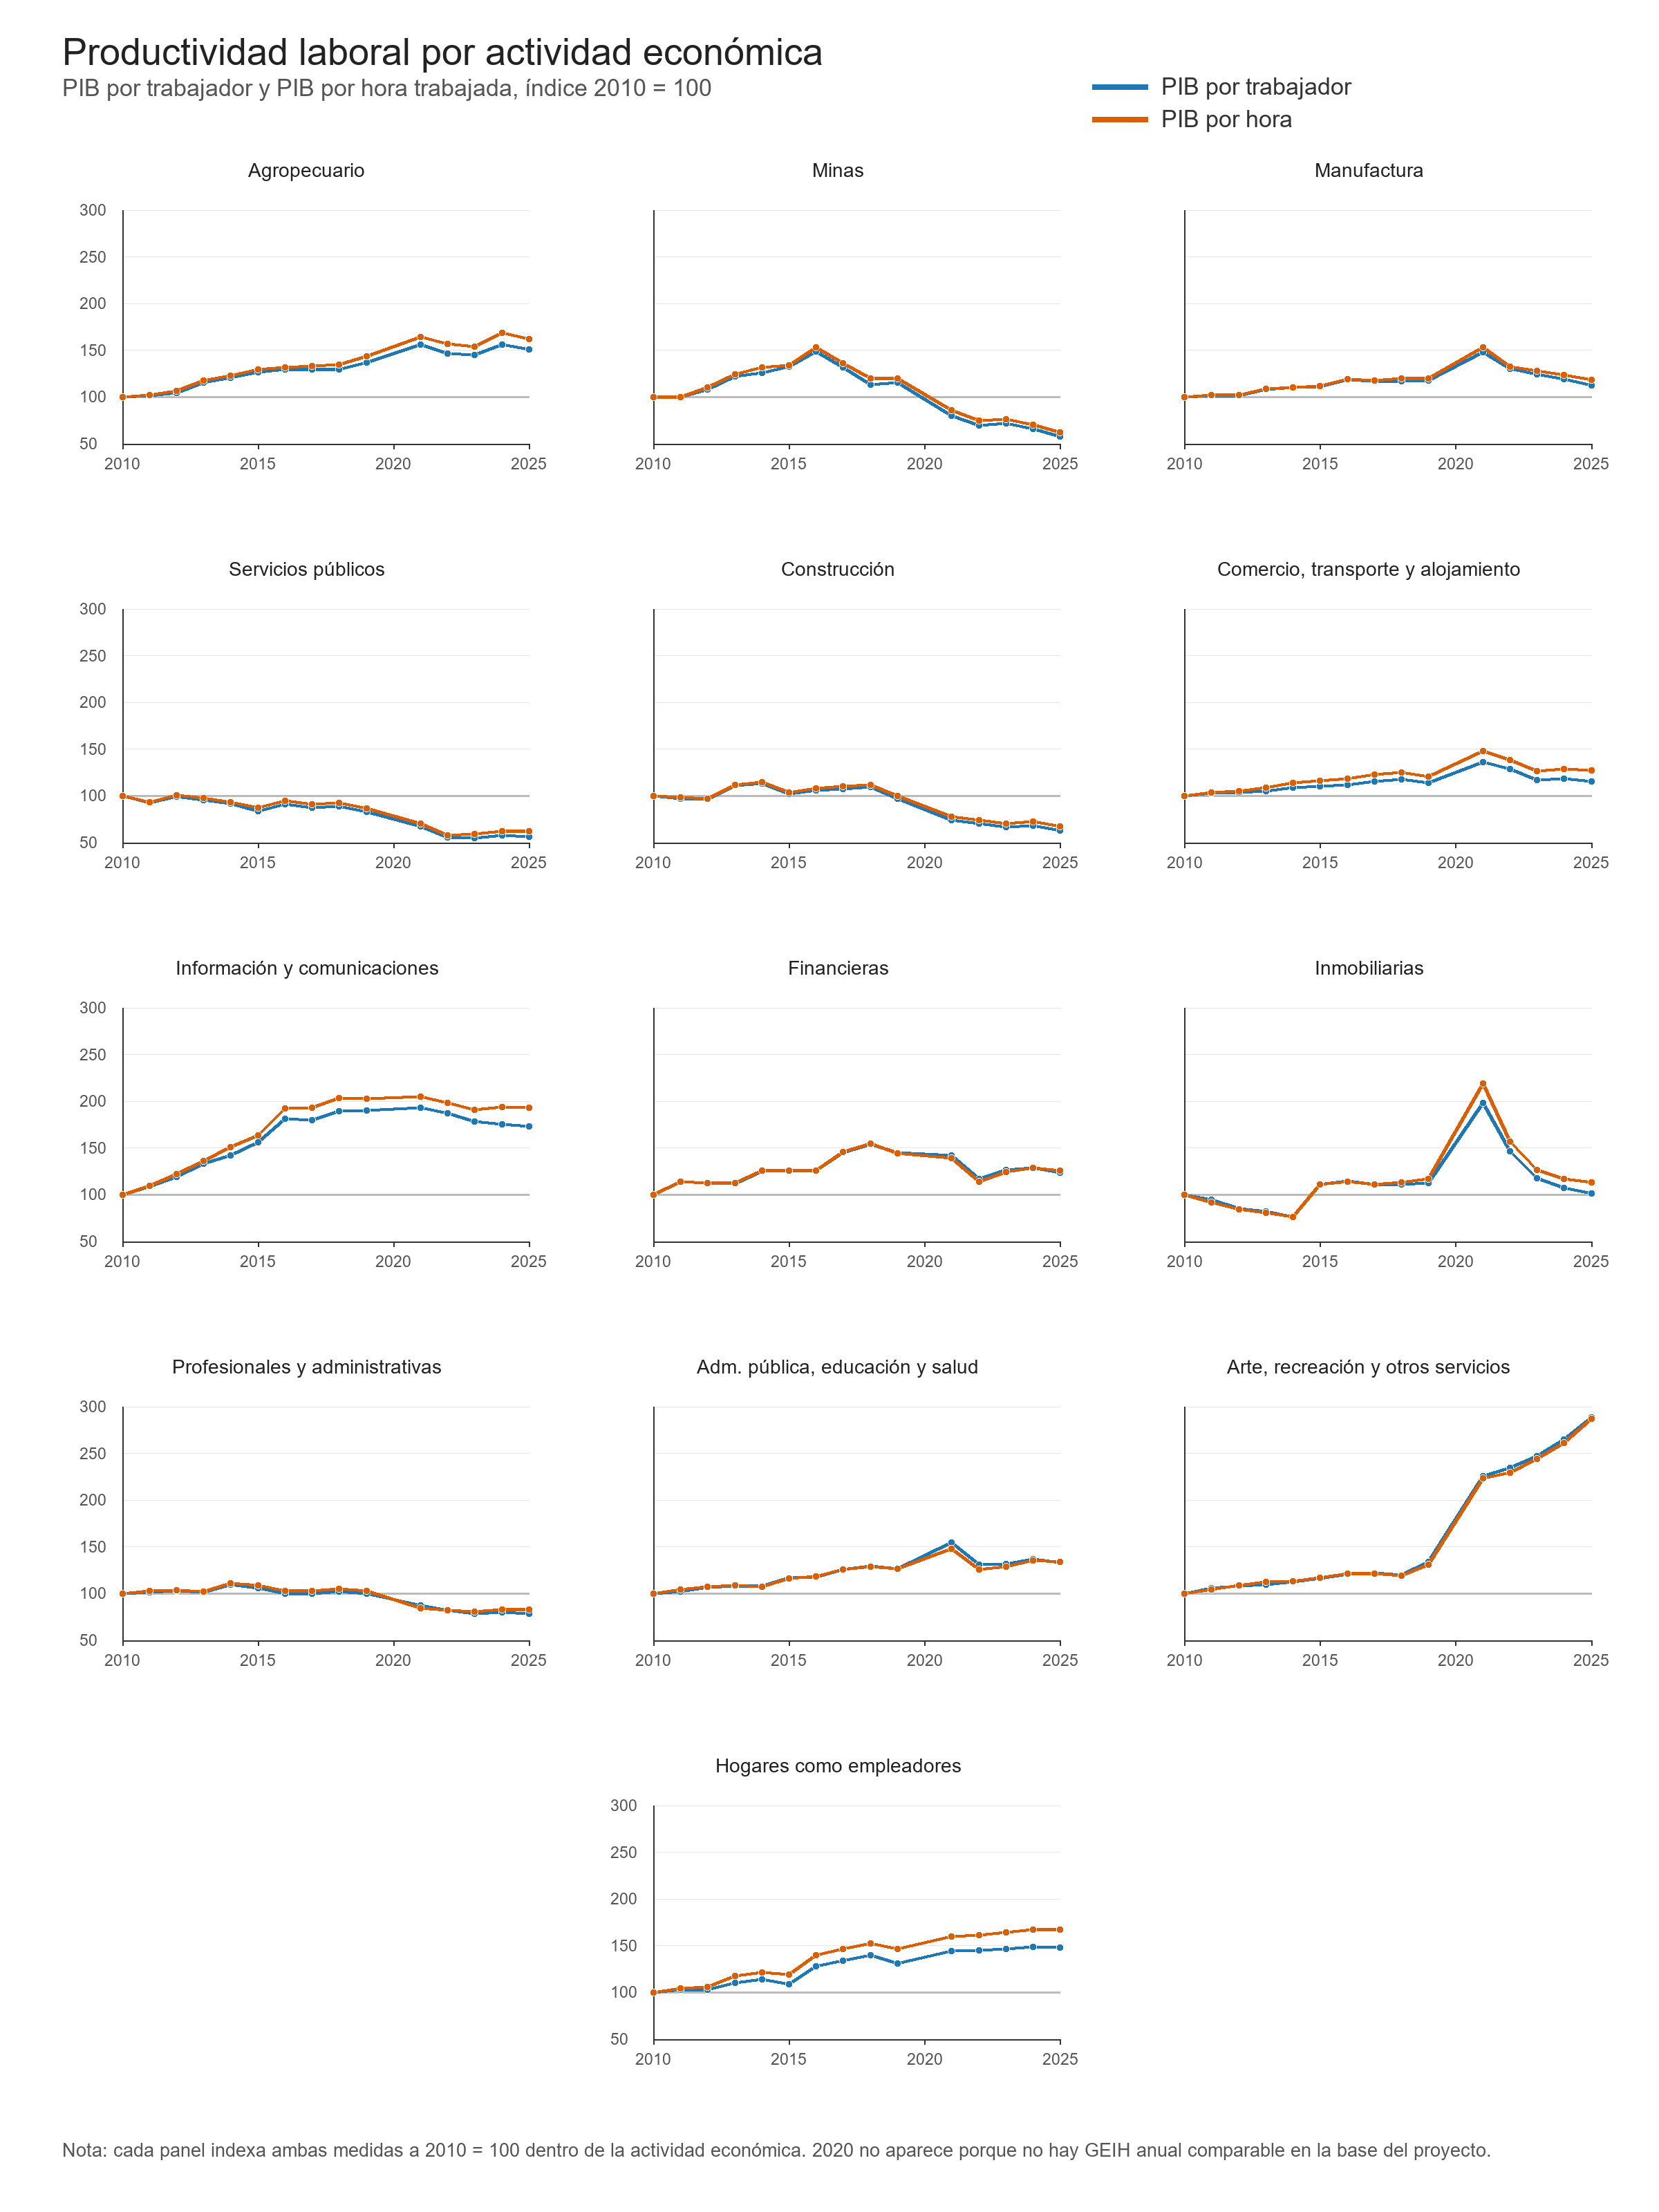
\includegraphics[width=1.03\textwidth]{Paper/figures/fig_pib_geih_productividad_sector_indices.png}}
  \caption{Productividad laboral por grandes ramas de actividad económica, índice 2010 = 100}
  \label{fig:pib_geih_productividad_sector_indices}
  \caption*{\footnotesize Nota: el PIB por trabajador y el PIB por hora trabajada se indexan a 2010 = 100. Fuente: cálculos propios con DANE y GEIH.}
\end{figure}

%El Cuadro \ref{tab:pib_geih_productividad_61} presenta una desagregación de las actividades económicas mayor a la del Cuadro \ref{tab:pib_geih_productividad_sector}. Cuando la GEIH no permite separar ocupados y horas con el mismo detalle, las subactividades del DANE aparecen agrupadas en la observación laboral comparable.


\begingroup
\footnotesize
\begin{longtable}{p{0.34\textwidth}rrrrrr}
\caption{Productividad laboral por subactividades, 2010--2025}\label{tab:pib_geih_productividad_61}\\
\toprule
& \multicolumn{3}{c}{PIB por trabajador} & \multicolumn{3}{c}{PIB por hora} \\
& \multicolumn{3}{c}{\footnotesize Millones de pesos de 2015} & \multicolumn{3}{c}{\footnotesize Miles de pesos de 2015} \\
\cmidrule(lr){2-4}\cmidrule(lr){5-7}
Actividad económica & 2010 & 2025 & Crec. & 2010 & 2025 & Crec. \\
\midrule
\endfirsthead
\toprule
& \multicolumn{3}{c}{PIB por trabajador} & \multicolumn{3}{c}{PIB por hora} \\
& \multicolumn{3}{c}{\footnotesize Millones de pesos de 2015} & \multicolumn{3}{c}{\footnotesize Miles de pesos de 2015} \\
\cmidrule(lr){2-4}\cmidrule(lr){5-7}
Actividad económica & 2010 & 2025 & Crec. & 2010 & 2025 & Crec. \\
\midrule
\endhead
Arte, recreación y otros servicios & 11,4 & 32,8 & 7,32\% & 5,6 & 16,0 & 7,28\% \\
Silvicultura & 33,1 & 70,2 & 5,15\% & 13,2 & 32,9 & 6,27\% \\
Pesca y acuicultura & 12,2 & 24,6 & 4,79\% & 4,7 & 10,9 & 5,75\% \\
Ganadería & 14,1 & 27,1 & 4,45\% & 5,7 & 12,0 & 5,10\% \\
Información y comunicaciones & 45,4 & 78,6 & 3,73\% & 17,6 & 34,0 & 4,49\% \\
Transporte aéreo & 183,2 & 286,1 & 3,02\% & 72,9 & 126,4 & 3,74\% \\
Impresión y reproducción & 29,4 & 44,8 & 2,85\% & 12,2 & 20,1 & 3,40\% \\
Hogares como empleadores & 6,4 & 9,4 & 2,63\% & 2,7 & 4,5 & 3,49\% \\
Salud y servicios sociales & 33,7 & 49,1 & 2,54\% & 14,7 & 21,3 & 2,47\% \\
Equipo eléctrico y electrónico & 39,0 & 56,0 & 2,45\% & 15,5 & 23,6 & 2,83\% \\
Comercio; Reparación de vehículos & 16,3 & 22,8 & 2,28\% & 6,3 & 9,5 & 2,76\% \\
Cultivos, apoyo agropecuario y mixtos & 14,7 & 20,5 & 2,24\% & 6,5 & 9,6 & 2,61\% \\
Almacenamiento y apoyo al transporte & 27,6 & 37,2 & 2,02\% & 10,7 & 15,8 & 2,59\% \\
Café & 7,2 & 9,3 & 1,75\% & 3,1 & 4,1 & 1,98\% \\
Textiles y confecciones & 16,5 & 21,3 & 1,70\% & 7,1 & 9,5 & 1,91\% \\
Vehículos y equipo de transporte & 48,5 & 62,4 & 1,70\% & 18,6 & 26,2 & 2,31\% \\
Alimentos, bebidas y tabaco & 40,1 & 50,9 & 1,61\% & 17,0 & 21,9 & 1,71\% \\
Educación de mercado; Educación de no mercado & 41,6 & 52,4 & 1,56\% & 21,4 & 25,8 & 1,27\% \\
Otras manufactureras & 32,8 & 41,2 & 1,53\% & 15,9 & 20,6 & 1,71\% \\
Financieras y seguros & 101,0 & 124,5 & 1,40\% & 43,0 & 54,2 & 1,56\% \\
Administración pública y defensa & 62,7 & 77,2 & 1,40\% & 23,7 & 32,2 & 2,06\% \\
Papel y cartón & 77,3 & 89,1 & 0,96\% & 30,6 & 37,6 & 1,37\% \\
Inmobiliarias & 280,0 & 284,6 & 0,11\% & 105,3 & 119,5 & 0,85\% \\
Petróleo, gas y apoyo conexo & 570,5 & 576,1 & 0,07\% & 211,9 & 231,6 & 0,59\% \\
Gas, vapor y aire acondicionado & 155,7 & 154,9 & -0,03\% & 61,4 & 64,5 & 0,33\% \\
Muebles y colchones & 13,8 & 13,6 & -0,09\% & 5,3 & 5,6 & 0,35\% \\
Energía eléctrica & 303,3 & 298,7 & -0,10\% & 118,9 & 125,0 & 0,33\% \\
Metalurgia y productos metálicos & 31,5 & 30,5 & -0,22\% & 12,3 & 12,8 & 0,25\% \\
Madera & 19,5 & 18,5 & -0,38\% & 8,5 & 9,6 & 0,81\% \\
Minerales no metálicos & 124,7 & 113,9 & -0,60\% & 47,8 & 47,8 & -0,01\% \\
Transporte terrestre y tuberías & 27,5 & 24,5 & -0,78\% & 8,9 & 9,3 & 0,33\% \\
Químicos y farmacéuticos & 97,7 & 86,3 & -0,82\% & 39,5 & 36,7 & -0,49\% \\
Otras minas y canteras & 52,2 & 45,6 & -0,89\% & 21,1 & 19,7 & -0,45\% \\
Coquización y refinación & 2.441,9 & 2.103,3 & -0,99\% & 933,9 & 882,8 & -0,37\% \\
Alojamiento y comida & 27,6 & 23,4 & -1,08\% & 11,4 & 10,7 & -0,42\% \\
Maquinaria e instalación & 44,8 & 38,1 & -1,09\% & 17,8 & 16,5 & -0,50\% \\
Caucho y plástico & 34,4 & 28,3 & -1,28\% & 13,3 & 11,7 & -0,83\% \\
Servicios administrativos y de apoyo & 43,9 & 36,0 & -1,32\% & 20,5 & 18,0 & -0,87\% \\
Profesionales, científicas y técnicas & 73,0 & 54,7 & -1,91\% & 32,1 & 25,2 & -1,60\% \\
Transporte acuático & 16,1 & 11,0 & -2,52\% & 6,0 & 4,6 & -1,76\% \\
Obras civiles & 83,2 & 56,2 & -2,58\% & 31,3 & 23,1 & -2,01\% \\
Aguas residuales, desechos y saneamiento & 118,8 & 73,3 & -3,17\% & 46,7 & 31,2 & -2,64\% \\
Agua & 61,1 & 37,6 & -3,19\% & 24,7 & 15,6 & -3,02\% \\
Actividades especializadas de construcción & 44,0 & 26,7 & -3,27\% & 18,3 & 11,7 & -2,90\% \\
Edificaciones & 34,1 & 19,9 & -3,52\% & 13,3 & 8,3 & -3,08\% \\
Correo y mensajería & 11,2 & 6,4 & -3,61\% & 4,5 & 2,7 & -3,41\% \\
Cuero, calzado y artículos de viaje & 12,5 & 6,5 & -4,31\% & 4,7 & 2,9 & -3,14\% \\
Carbón & 256,7 & 103,5 & -5,88\% & 95,1 & 41,8 & -5,33\% \\
Minerales metalíferos & 47,7 & 17,6 & -6,44\% & 18,8 & 7,5 & -5,98\% \\
Reciclaje & 462,1 & 14,9 & -20,45\% & 197,5 & 7,2 & -19,83\% \\
\bottomrule
\end{longtable}
\endgroup
{\footnotesize Nota:  A nivel de actividad económica, el numerador de los indicadores de productividad corresponde estrictamente al valor agregado bruto de cada actividad. El renglón Alimentos, bebidas y tabaco agrega manufacturas de carnes y pescado, aceites, lácteos, molinería y panadería, café, azúcar y panela, cacao y confitería, frutas y hortalizas, otros alimentos, bebidas y tabaco. Fuente: cálculos propios con DANE y GEIH.}
